\subsection{Local Outlier Factor}
\label{section:LOF}

\begin{figure}[t]
    \centering
    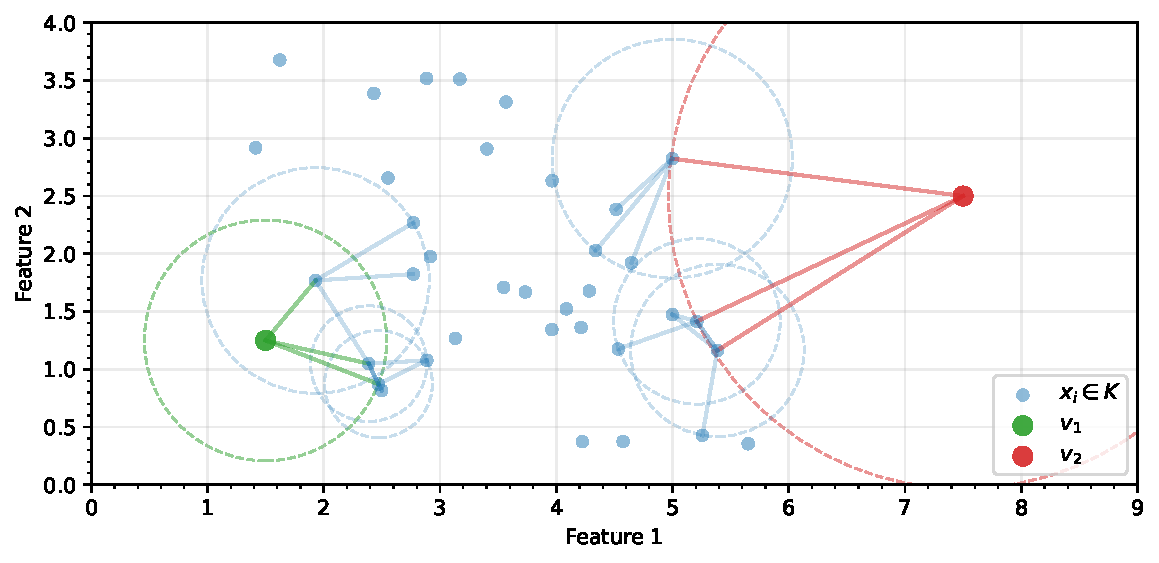
\includegraphics[width=\textwidth]{images/measures/lof-distance.pdf}
    \caption{Idea of the Local Outlier Factor applied as an outlierness measure. \\
             The $k=3$ closest neighbors are considered when identifying the reachability distances (represented as the radiuses of circles).
             For element $v_1$ the reachability distance is~similar as for it's neighbors,
             whereas for element $v_2$ it is significantly greater.}
    \label{fig:lof-idea}
\end{figure}

The Local Outlier Factor (LOF), originally described by Breunig et al. \cite{Breunig-2000}, is a well-established algorithm widely used to detect abnormal data in high-dimensional spaces. It is based on the concepts of so called reachability distance and local reachability density. Instead of considering the global data distribution, it aims to identify outliers by analyzing only the local neighborhood. Hence, it can be considered as an extension of the k-Nearest Neighbors algorithm.

Let $N_k(v, T)$ be a function that returns the set containing $k$ number of elements $x_i$ from cluster $T$ that are closest to $v$. The base concepts utilized by LOF are therefore defined as follows. First, the $kdist(v, T)$ is defined as the distance from given $v$ to its $k$-th neighbor from the cluster $T$,
\begin{equation}
    kdist(v, T)
    =
    \max\big\{
        ~
        \forall x_i \in N_k(v, T): ~ \norm{\vv{v - x_i}}
        ~
    \big\}
    .
    \label{eq:kdist}
\end{equation}

Then, the reachability distance of element $v$ with respect to the element $x$ and cluster $T$ is defined as either the true distance between $v$ and $x$, or as the $kdist(x, T)$ distance of element $x$, whichever turns greater,
\begin{equation}
    rd_k(v, x, T)
    =
    \max\big\{
        ~
        kdist(x, T),
        ~
        \norm{\vv{v - x}}
        ~
    \big\}
    .
\end{equation}

Successively, the local reachability density for an element $v$ with respect to the given cluster $T$ is defined as the inverse of the average reachability distance of element $v$ and its $k$ neighbors from set $T$,
\begin{equation}
    lrd_k(v, T)
    =
    \frac{
        k
    }{
        \sum_{x_i \in N_k(v, T)} rd_k(v, x_i, T)
    }
    ~.
\end{equation}

Finally, the outlierness score for a given vector $v$ against the target data cluster $T$ is calculated as an average local reachability density of $k$ neighbors of $v$, divided by the local reachability density of the $v$ element,
\begin{equation}
    LOF(v, T)
    =
    \frac{
        \sum_{x_i \in N_k(v, T)} lrd_k(x_i, T)
    }{
        k \cdot lrd_k(v, T)
    }
    ~.
\end{equation}

Figure \ref{fig:lof-idea} illustrates the idea of Local Outlier Factor algorithm. Intuitively, the algorithm compares the radiuses of circles corresponding to the reachability distances of the analyzed points and their $k$ closest neighbors. Shall these radiuses be similar to their neighbors ones ($v_1$, score $LOF \approx 1$), the point can be considered an inlier. On~the~other hand, when the radius at analyzed point is much greater ($v_2$, $LOF \gg 1$), then such point is likely an outlier. High score value means a given point $v$ is relatively far from the cluster, as there is low density of points in the surrounding area (inverse of reachability distance).

It is worth to mention that, similarly to k-Nearest Neighbors algorithm, the Local Outlier Factor does not require any \textit{a priori} assumption on the data distribution, since it identifies the outliers only by analyzing the local surroundings of data. Hence LOF algorithm represents so called non-parametric approach to anomaly detection.

The LOF algorithm captures the intuition that outliers are isolated points, while denser regions of data are related with areas typical for a given distribution. It can be adapted to handle different distance metrics as well. Nevertheless, the value of $k$ affects the sensitivity of the algorithm to any local variations in density. However, the algorithm can be computationally expensive for large datasets due to the complexity of finding neighbors in data.

During the research the implementation from the scikit-learn library \cite{scikit-learn} was utilized.
